\section{Condición I} 
\vspace{16mm} %5mm vertical space
\begin{center}
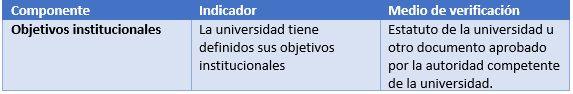
\includegraphics[width=17cm]{./Imagenes/001}
\end{center}	
\vspace{12mm} %5mm vertical space

\textbf{Condición I. Existencia de objetivos académicos, grados y títulos a otorgar y planes de estudio correspondientes.}

Objetivo:
Internalizar en la comunidad universitaria (autoridades, docentes, administrativos y estudiantes) la información que posee y acciones que viene implementando la Universidad Peruana Los Andes con la finalidad de lograr satisfactoriamente su proceso de licenciamiento a través de las ocho condiciones básicas de calidad.\\
Aspecto General del Proceso de Licenciamiento\\
\\
1.	El cumplimiento de las Condiciones Básicas de calidad.\\
2.	Etapas que contempla en proceso de licenciamiento.\\
3.	Otorgar la licencia de funcionamiento institucional a las Universidades.\\
4.	Qué universidades están obligadas a obtener licencia de funcionamiento institucional.\\


\textbf{Condición I: Existencia de objetivos académicos, grados y títulos a otorgar y planes de estudio correspondientes.}\\
-	Según la Ley 30220 y de acuerdo al estatuto de la Universidad Privada de Tacna, reemplazar en sus funcionales del Vicerrectorado Administrativo.\\
-	De acuerdo al estatuto de la Universidad Peruana Los Andes. Propone al Consejo de Facultad la contrata de docentes mediante proceso de selección; 		asimismo la separación en caso de cometer falta grave.\\
-	De acuerdo al estatuto de la Universidad Peruana Los Andes, La universidad se organiza por facultades que son unidades de formación académica, 		profesional y de gestión. Ordene en forma jerárquica: a) Unidades de investigación, b) Los Departamentos Académicos, c) Unidades de posgrado y d) 		Escuelas Profesionales.\\
-	Los estudios generales, los estudios específicos y de especialidad. Tienen una duración mínima de cinco (5) años, los que se realizan en dos semestres     	académicos por año. El enunciado comprende a:\\
-	Para estudios presenciales se define un crédito académico como equivalente a un mínimo de:\\
-	El Plan de estudios de la Escuela Profesional de Administración y Sistemas cumple con los créditos necesarios de pregrado que exige la Ley 30220 para 		el funcionamiento de una carrera, teniendo un total de créditos de: \\
-	El Plan de estudios de la Escuela Profesional de Contabilidad y Sistemas cumple con los créditos necesarios de pregrado que exige la Ley 30220 para el 		funcionamiento de una carrera, teniendo un total de créditos de:\\
-	Los egresados que hayan obtenido el Grado Académico de bachiller pueden obtener el título profesional mediante las siguientes modalidades\\




